\chapter{Cortex Neuron Network}

In the cortex, the timing of successive action potentials is highly irregular.
Then, the irregular interspike interval reflects a random process and implies
that an instantaneous estimate of the spike rate can be obtained by averaging
the pooled responses of many individual neurons.


\section{Spike generation}

Spike generation refers to the activation of AP at the soma axon hillock.
The poisson  model provides a good description of some data
(Sect.\ref{sec:spike-Poisson}).
However, it does not provide the proper mechanistic explanation of neuronal
response variability. As in vitro, the spike generation is very reliable, and
deterministic, Fig.\ref{fig:spike-generation}(A), yet in vivo, it is quite
random. This is believed to be the result from the fact that synapses are very
unreliable , not the spike generator. So, it is important to understand the
change in synaptic plasticity at synapse level.



\begin{figure}[hbt]
  \centerline{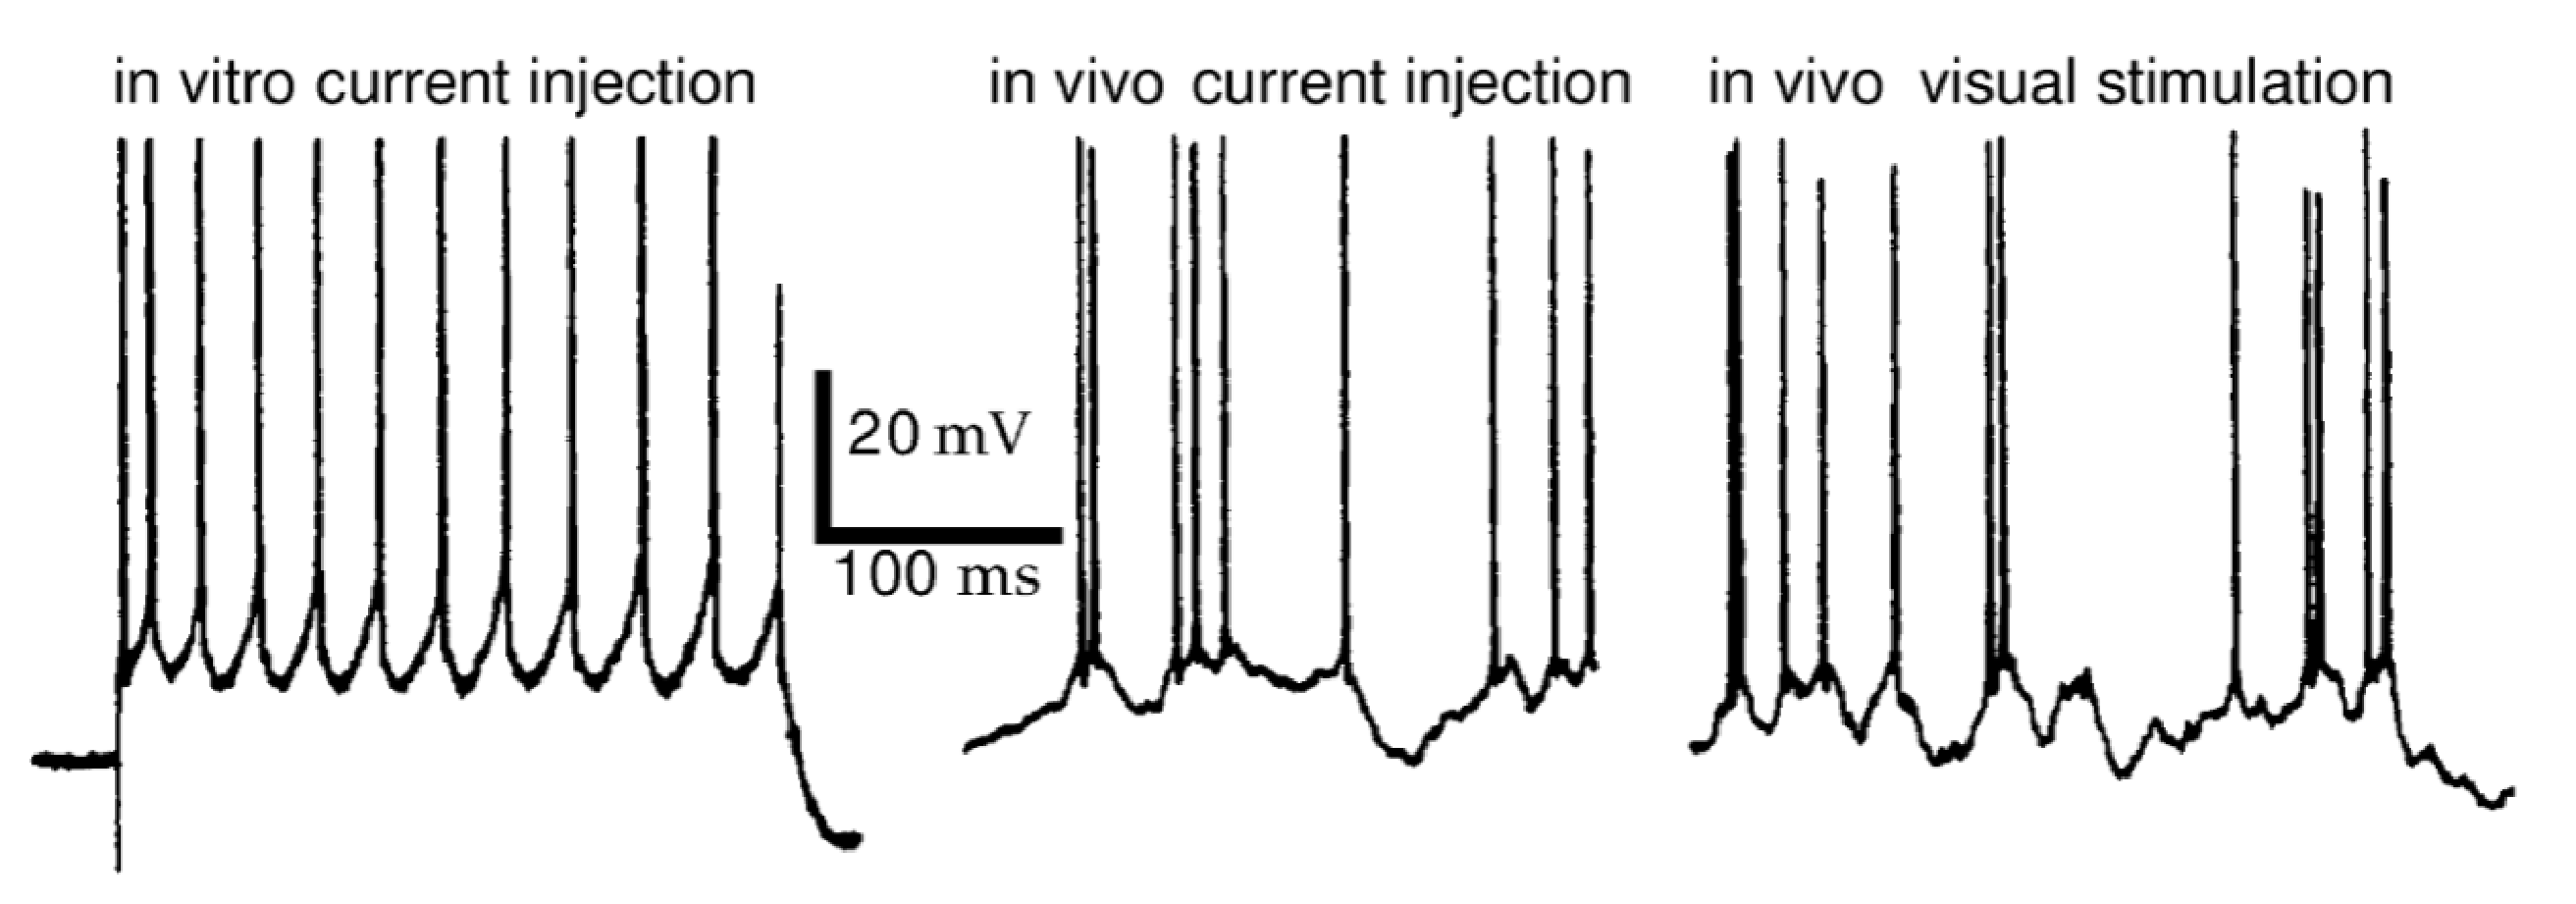
\includegraphics[height=5cm,
    angle=0]{./images/spike-generation.eps}}
  \caption{Spike generation: (A) {\it in vitro}; (B) {\it in vivo}}
  \label{fig:spike-generation}
\end{figure}


\section{Indepenent spike hypothesis: Poisson behavior of firing}
\label{sec:spike-Poisson}

It is assumed that regardless of the stimulus, the generation of spike is a
stochastic process. In other words, we assume that the generation of each spike
depends only on an underlying continuous/analog driving signal, r(t), that we
will refer to as the instantaneous firing rate.
It follows that the generation of each spike is independent of all the other
spikes , hence we refer to this as the {\bf independent spike hypothesis}.

If the independent spike hypothesis were true, then the spike train would
be completely described a particular kind of random process called a {\bf
Poisson process}, Fig.\ref{fig:Poisson-process_cortex_spike}.


\begin{figure}[hbt]
  \centerline{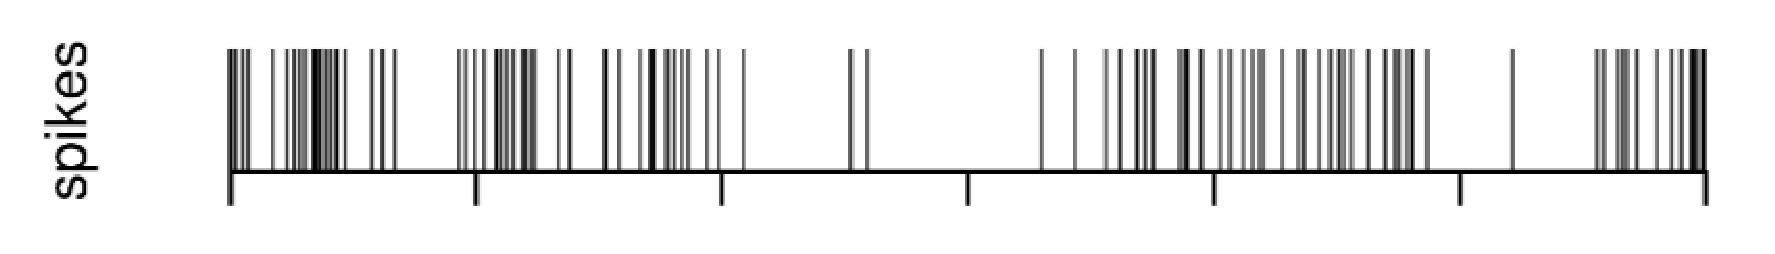
\includegraphics[height=2cm,
    angle=0]{./images/Poisson-process_cortex_spike.eps}}
  \caption{Spikes generated from a Poisson process}
  \label{fig:Poisson-process_cortex_spike}
\end{figure}

The probability for a spike to occur within an interval $\Delta t$ based on the
probability density p[t] is
\begin{equation}
P = p[t] \times \Delta t
\end{equation}

Suppose a spike train consists of $n$ spikes: for a spike train at $n$ time
points $(t_1,t_2,\ldots,t_n)$.
Among all spike trains of $n$ spike, what is the probability
$P[t_1,t_2,\ldots,t_n]$ for the spike train $(t_1,t_2,\ldots,t_n)$ to occur?


% ; then the probability density is denoted as
% $p[t_1,t_2,\ldots, t_n]$.

%ASSUMPTION: An action potential is independent of the presence of other spikes.

\subsection{Homogeneous Poisson process}

Assume the average firing rate of a cell is constant: $r(t) = r$ (e.g. 100
spikes per second).
If we devide the time interval $T$ into $M$ bins of width $\Delta t = T/M$. If
$\Delta t$ is small enough that we never get two spikes within any one bin.
So, the probability for a single spike occuring in an interval is $r.\Delta t$.
The probability of not having a spike in a given bin is $(1-r\Delta t)$.

The probbaility of having $(M-n)$ bins without spikes is 
$(1-r\Delta t)^{(M-n)}$. The number of ways selecting $n$ bins out of $M$ bins
is given by the binomial coefficient
\begin{equation}
\frac{M!}{(M-n)! n!}
\end{equation}

So, with $n$ spikes that arranges into $M$ bins, the number of ways putting
these $n$ spikes into the $M$ bins is a combinatorial factor.
Then, it can be expressed by a probability function that considers only the
number of spikes $P_T[N]$ within the duration $T$.


\begin{equation}
P_T[n] = \lim_{\Delta \rightarrow 0} \frac{M!}{(M-n)! n!}
\left( r\Delta t\right)^n \left( 1-r\Delta t\right)^{(M-n)}
\end{equation} 

If $M$ grows without bound, and $n$ is fixed, then 
\begin{enumerate}
  \item  $M-n \approx M = T/\Delta t$.

  \item $\frac{M!}{(M-n)! n!}  \approx M^n = (T/\Delta t)^n$

NOTE: $\lim_{\varepsilon \rightarrow 0 } \left( (1+\varepsilon)^{1/\varepsilon}\right) = \varepsilon$

\end{enumerate}
then
\begin{equation}
P_T[n] \approx \frac{(T/\Delta t)^n}{n!} (r\Delta t)^n \varepsilon^{-rT} 
  = \frac{(rT)^n}{n!} \varepsilon^{-rT}
\end{equation}
which is a Poisson distribution, Fig.\ref{fig:Poisson_distribution}.


% So, 
% \begin{equation}
% P_T[n] = 
% \end{equation}
% 
% So,
% $P_T[n]$ is the 
% 
% So, the probability for
% a
% % single
% spike train


\begin{figure}[hbt]
  \centerline{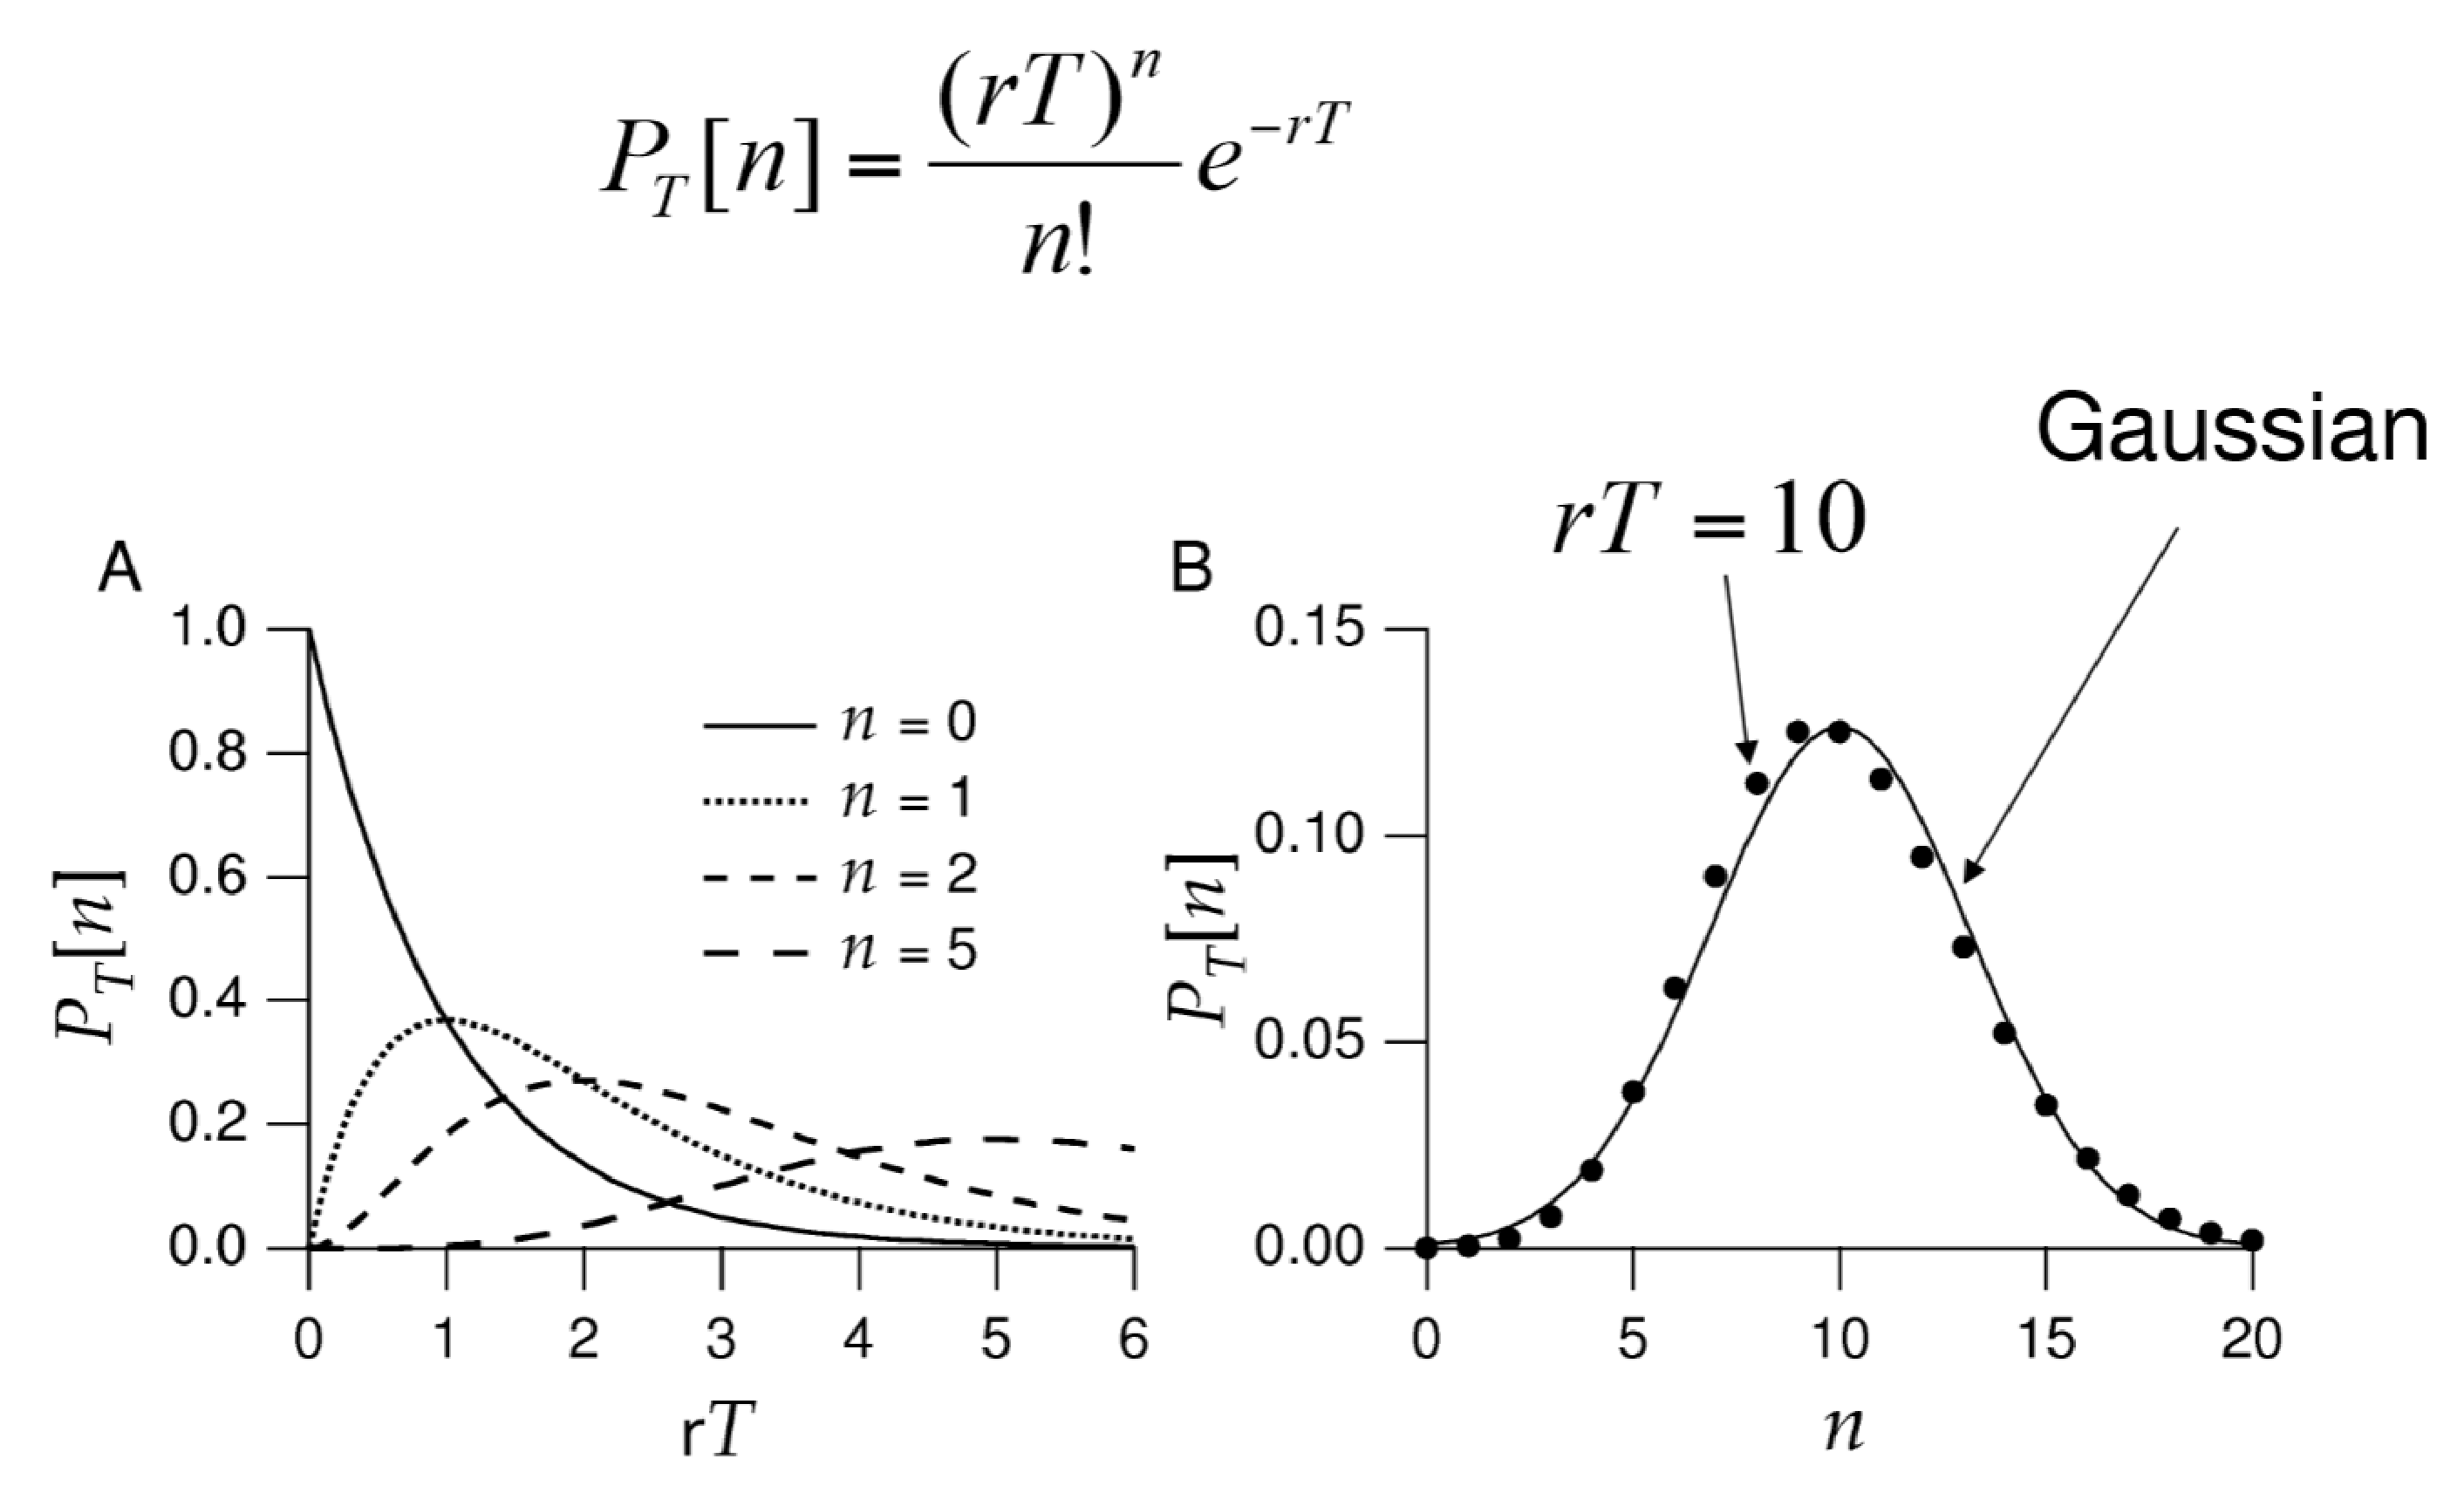
\includegraphics[height=5cm,
    angle=0]{./images/Poisson_distribution.eps}}
  \caption{Poisson distribution with different values of $n$ as the number of
  spikes in the time interval $T$; (B) Gaussian distribution}
  \label{fig:Poisson_distribution}
\end{figure}

\subsection{Poisson spike generator}

\def\rand{{\text{rand}}}


\subsection{ * discrete time bin}

To generate stochastic spike based on Poisson process, a program that progresses 
in time through small time steps $\Delta t$ (e.g. 1ms), and each time step,
generate a random variable $x_\rand$ between 0 and 1; and use this test for determining of
a spike occurs in that time step or not

\begin{equation}
r_i \Delta t \left\{ 
\begin{array}{cc}
> x_\rand & fire a spike \\
\le x_\rand & nothing
\end{array} 
\right.
\end{equation}

\section{recurrent sparsely connected neural network}
\label{sec:cortical-network-AMPA-GABA}

A recurrent sparsely connected neural network of leaky integrate and fire
(LIF) neurons (Tuckwell, 1988; Brunel and Wang, 2003). 

Suppose we have a network with 4000 pyramidal neurons with AMPA-like synapses,
and 1000 interneurons with GABA-like synapses. Each neuron is modeled using IaF
(Sect.\ref{sec:Integrate-and-Fire-Spike}). The network connectivity was random
and sparse, with a connection probability of 0.2 between any pair of cells
(Mazzoni et al., 2008; Mazzoni et al., 2010).

AMPA and GABA postsynaptic currents were determined by the spikes emitted by the
pre-synaptic neurons of the network and by the external inputs mimicking the
thalamic inputs (conveying the information about sensory stimuli) and the
ongoing cortical fluctuations (summarizing the effect of the slow covariations
in network state due to ongoing activity)
